\documentclass{article}
\usepackage{graphicx}
\usepackage[a4paper, hmargin = 2.5cm, vmargin = 2.5cm]{geometry}
\usepackage[english]{babel}

\title{Datenbankprojekt : Reisebüro/Travel agency}
\author{Oliver Baltisberger, Rachid Flueckiger, Christian Pernet}
\date{\today}

\begin{document}
	\maketitle
	
	\section*{Project description}
	Our project aims to implement a (very) simple customer relationship management 
	database for a travel agency. 
	Several travel agencies employ collaborators. These employees sell trips to 
	customers. 
	In our example, the trips are organized trips. They also have a begin date, a 
	duration, a price and a category. 
	The category can be e.g. cruse, road trip, safari, ...
	
	\section*{Queries examples}
	
	\subsection*{Christian}
			\begin{enumerate}
				\item make a list of all employees.
				\item make a list of all employees working for a particuliar agency.
				\item count the number of trips sold by an employee.
				\item which employee has sold the highest number of trips.
				\item sum the sales made by an employee
				\item make a list of the clients.
				\item determine the preferred paiement method of the clients.
				\item determine the preferred contact method of the clients.
				\item make a list of the trips.
				\item make a list of the trips for a particuliar category.
				\item make a list of the clients who have reserved a trip.
				\item for each category, list all the reservation made by clients.
				\item determine for a sale, if the paiement is complete.
			\end{enumerate}
	
	\subsection*{Oliver}
			\begin{enumerate}
				\item Make a list of all trip themes (e.g. mountains, city, beach, countryside)
				\item Make a list of all destination countries = locations (e.g. Switzerland, Spain, Italy, France, USA)
				\item Make a list of all trips suited for a specific customer group (e.g families, couples, singles)
				\item Make a list of all accomodation types (e.g. hotel, vacation homes)
				\item List all destinations (e.g. Mallorca, London, Turkey, Florida) sorted by popularity
				\item List all employees and the number of trips they have sold in the last 12 months
				\item List number of trips sold online and offline (i.e. sold in a travel agency)
				\item List most popular months of travel (e.g. more trips in July than in November)
				\item List popular destinations per month of travel (e.g. July: Spain, Italy; December: Switzerland)
				\item What is average duration/price/numer of persons of a trip?
				\item What type of accomodation/transport/activity types are most popular?
				\item Do more experienced employees sell more trips?
				\item What is the preferred type of payment for trips?
			\end{enumerate}
			
\subsection*{Rachid}
			\begin{enumerate}
					\item Wer hat wie viele Reisen gebucht?
					\item Welche Übernachtungsmöglichkeit ist in welcher Saison beliebt bzw. unbeliebt?
					\item Häufigste Zahlungsmethode?
					\item Welcher Angestellter hat am meisten Reisen verkauft?
					\item wie viele Reisen wurden durschschnittlich in jeder Saison gebucht?
					\item Welche Kunden sind säumige Zahler?
					\item Welches Transportmittel wird am meisten/wenigsten benutzt?
					\item Welches Reiseziel ist das beliebteste/unbeliebteste?
					\item Alle Kunden, die in der selben Saison dasselbe Reiseziel haben.
					\item Alle Reisen, die entweder ohne Transportmittel oder Übernachtung gebucht worden sind.
				\end{enumerate}	
				
	\hrule
	\vspace{2 cm}
	On the next page, you find the ER-Diagram of this project. 
	
	
	\newpage
	
	\section*{ER-Diagram}
	\begin{figure}[htbp]
		\centering
			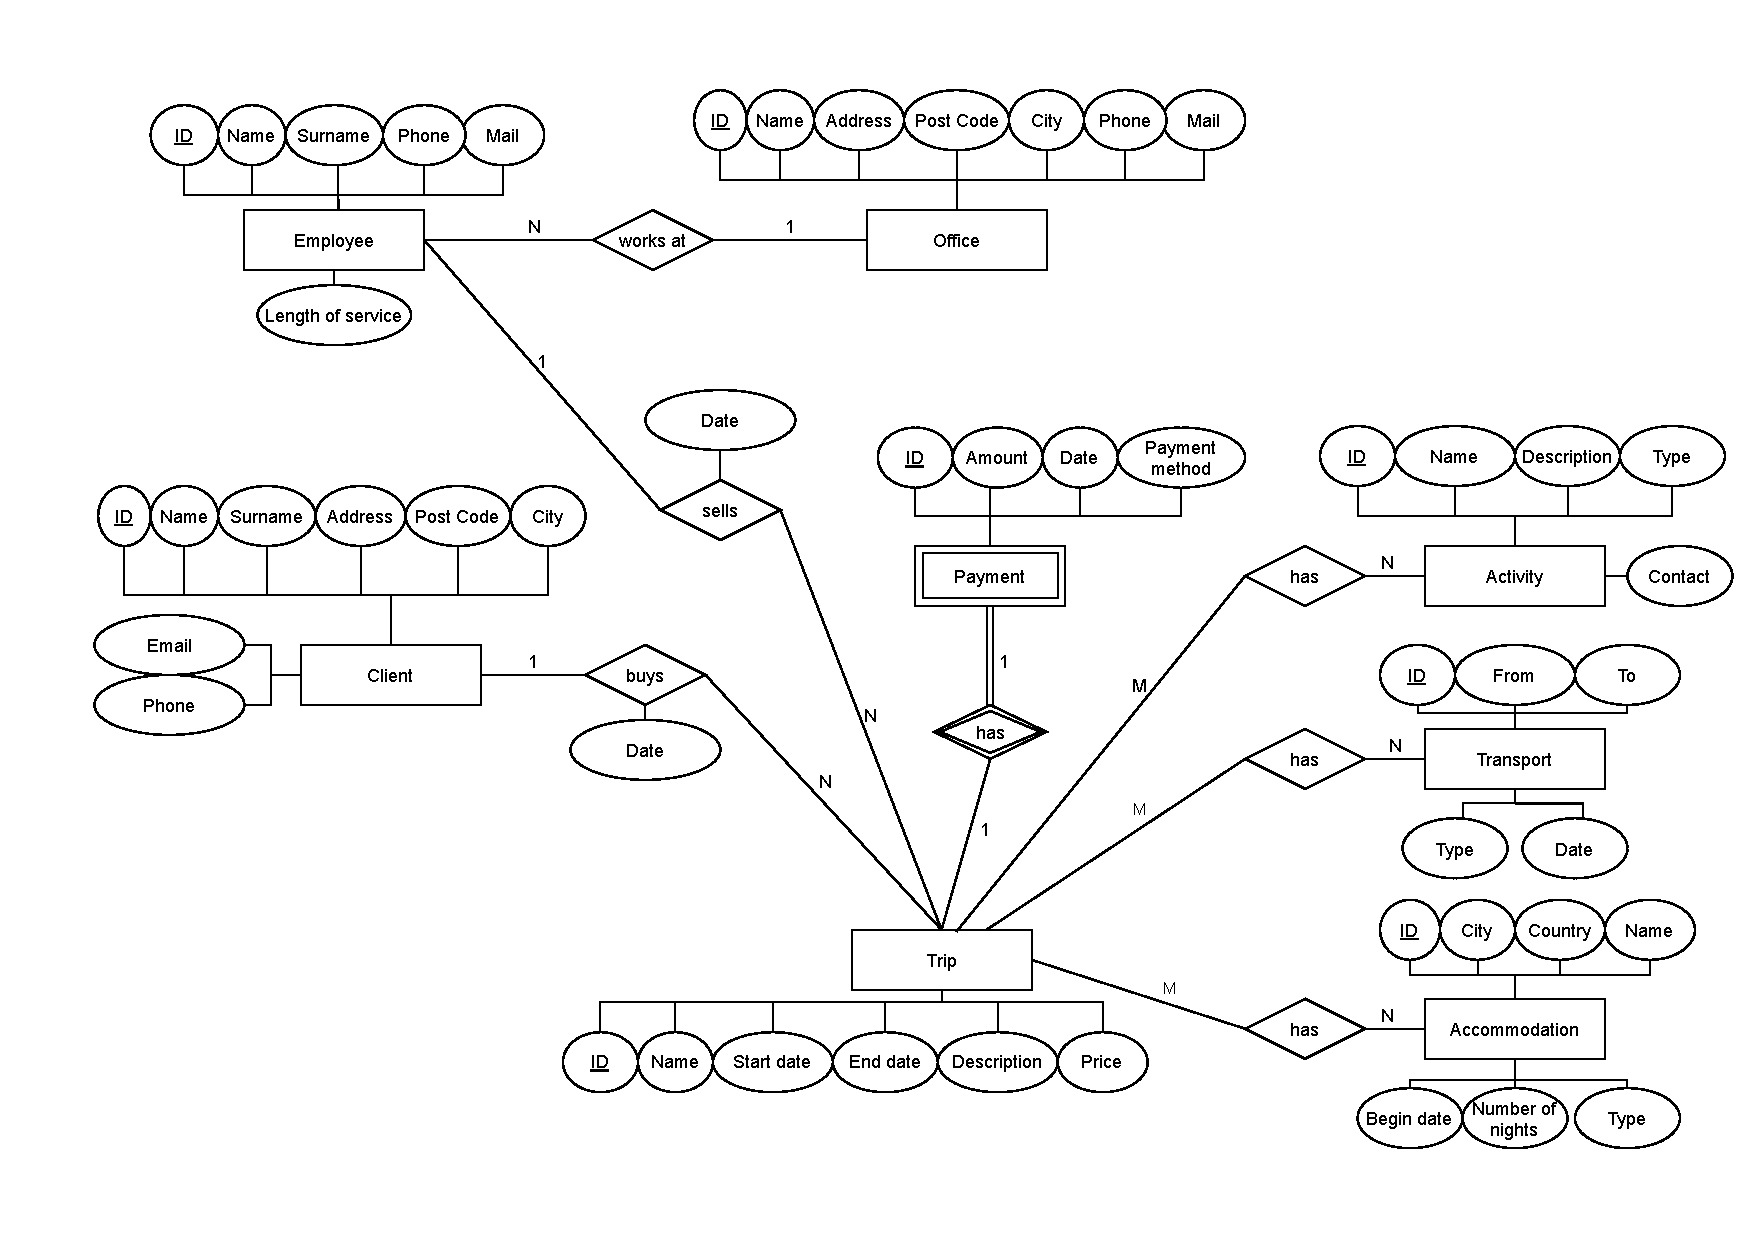
\includegraphics[width=1.15\textwidth, angle=90]{../Proposition 2.pdf}
		\label{ER-Model}
		\caption{Travel agency ER-Model}
	\end{figure}
	

\end{document}